\section{Introduction}

\subsection{Basic Concepts}

The greatest common divisor (GCD) of non-zero elements $a_1, \dots{}, a_n$ of an integral domain is defined as an element $g$, which and only which has the following properties:

\begin{enumerate}
    \item $g$ divides $a_1, \dots{}, a_n$ and
    \item every divisor of $a_1, \dots{}, a_n$ divides $g$.
\end{enumerate}Euclid's algorithm can be used to compute the GCD of two positive integers $a_1$ and $a_2$. It establishes the integer remainder sequence (IRS) \mbox{$a_1, a_2, \dots{}, a_k$}. By dividing $a_{i-2}$ by $a_{i-1}$, for \mbox{$i = 3, \dots{}, k$}, the IRS is constructed by the remainders of that division $a_i$:

\begin{align}
a_i = a_{i-2} - q_i \cdot a_{i-1} \qquad \text{for }  i = 3, \dots{}, k.
\end{align}The  Bézout cofactors $s$ and $t$ can also be used to calculate the GCD of $a_1$ and $a_2$:

\begin{align}
\text{gcd}(a_1, a_2) = s \cdot a_1 + t \cdot a_2.
\end{align}If the GCD of two integers $a_1$ and $a_2$ is 1, then the integers are said to be relatively prime or coprime. In this case \mbox{$s \cdot a_1 + t \cdot a_2 = 1$}. From this we immediately see that $s = a_1^{-1}\text{ mod }a_2$ and $t = a_2^{-1}\text{ mod }a_1$.

\subsection{Modular algorithms}

Sometimes it is easier not to solve a problem directly, but to transform it into another domain, solve the corresponding problem in that domain and transform the result back to the original domain. This is the basic idea of the modular method in computer algebra: A set of primes $p_1, \dots{}, p_m$ with respective homomorphisms $\phi_{p_1}, \dots{}, \phi_{p_m}$ is chosen and the problem is converted to a set of problems modulo different primes. These simpler problems are solved in $\mathbb{Z}_{p_1}, \dots{}, \mathbb{Z}_{p_m}$. Finally, the partial solutions are combined by the Chinese remainder algorithm \cite{winkler1996}:

\begin{table}[H]
\centering
\begin{tabular}[h]{rcccl}
& $\mathbb{Z} \times \mathbb{Z}$ & $\xrightarrow{\phi_{p_i}}$& $\mathbb{Z}_p \times \mathbb{Z}_p$ & \\
GCD in $\mathbb{Z}$ & $\downarrow$ &  & $\downarrow$ & GCD in $\mathbb{Z}_{p_i}.$ \\
& $\mathbb{Z}$ & $\xrightarrow{\phi_{p_i}}$ & $\mathbb{Z}_p$ & \\
\end{tabular}
\end{table}

\noindent While the conversion to the modular representation and the combining of the results incurs an additional overhead, solving many problems in modular representation may be significantly easier than solving the corresponding problem in the original domain. In particular, the complexity in the modular representation is less affected by the size of the problem. Consequently, the modular method provides algorithms with extremely good complexity behavior.

It could happen that an unlucky prime was chosen, for which the GCD of \mbox{$a$ mod $p$} and \mbox{$b$ mod $p$} is different from the modular image of the integer GCD of $a$ and $b$. For example, the GCD of the polynomials $a = x + 2$ and $b = x - 3$ is 1 over $\mathbb{Z}$. However, in modulo 5 representation $a$ and $b$ are equal, and their GCD is \mbox{$x + 2 \equiv x - 3$ mod $5$}. Fortunately, there are only finitely many unlucky primes to choose from and they are rare.

\subsection{Outline}

The remainder of this article is organized as follows:
The next section gives an overview of the modular algorithm and theory for integers.
The modular algorithm and theory for univariate and multivariate polynomials is introduced in section~\ref{Modular GCD of polynomials}.
Section~\ref{results} describes our results and concludes this article.

\section{Modular Algorithm for Integers}

This section introduces a modular algorithm for integers. The described algorithm follows to a great extent the publication by Kenneth Weber et al.\cite{modularInteger}.

\subsection{Introduction}

Computing the GCD of two integers can be more efficient and much faster using the modular representation than in the original representation. This is because in the modular representation the given problem can be solved by calculating with lower numbers than the original input size. Effectively, this prevents the necessity for specialized big integer data types, making it feasible to solve the problem with standard integer data types supported by the hardware. In particular, input sizes up to $2^{16} = 65{,}536$ bits can be handled using a set of $2^{17} = 131{,}072$ moduli between $2^{31}$ and $2^{32}$ \cite{modularInteger}.

On the other hand, converting the problem into modular representation incurs many computationally expensive division and modulo operations. However, certain arithmetic operations can be performed in parallel, each processor performing the operation modulo a separate prime simultaneously. This makes the modular integer GCD algorithm particularly interesting for concurrent read, concurrent write, parallel random access machines (CRCW PRAM) \cite{modularInteger}. On such a computational model, most of the modulo operations can effectively be performed in $O(1)$, mitigating the incurred additional cost of the modular representation.

Two variants of the algorithm are presented. The basic algorithm suppresses the modular representation for clarity and will also be used as a reference to demonstrate the benefit of the modular method. The modular algorithm extends the basic algorithm by converting the problem into the modular representation, solving the set of modular problems and converting the partial solutions back.

\subsection{Basic algorithm}

\begin{figure}
\caption{Basic algorithm of modular GCD computation of integers~\cite{modularInteger}.}
\centering
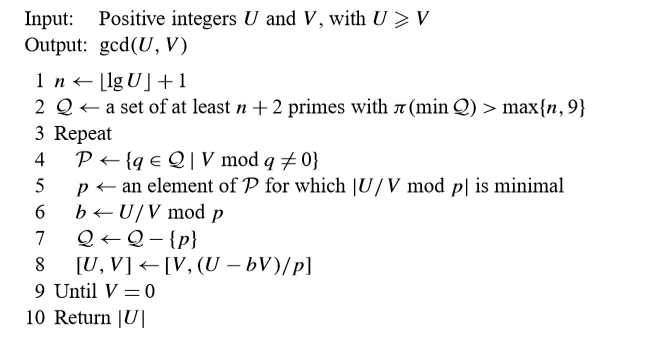
\includegraphics[scale=0.6]{texfiles/Integer_mod_basic.PNG}
 \label{fig:BasicAlgorithm}
\end{figure}

The basic algorithm as described by Weber et al.\ is depicted in Figure~\ref{fig:BasicAlgorithm}. First, we need to select a set of suitable primes $\mathcal{P}$. The primes are selected such to ensure that the reduction loop will terminate within at most \mbox{$n + 2$} iterations. After the selection, the reduction loop is entered. During each iteration the input integers $a$ and $b$ ($U$ and $V$ in Weber's notation) are reduced using one of the \mbox{$a / b\text{ mod }p$} \mbox{($p \in \mathcal{P}$)} values that is smallest in absolute value. This reduction step is repeated until $b$ is zero. The final value of $a$ is returned as the GCD of the input $a$ and $b$.

\subsection{Modular algorithm}

\begin{figure}
\caption{Final algorithm of modular GCD computation of integers~\cite{modularInteger}.}
\centering
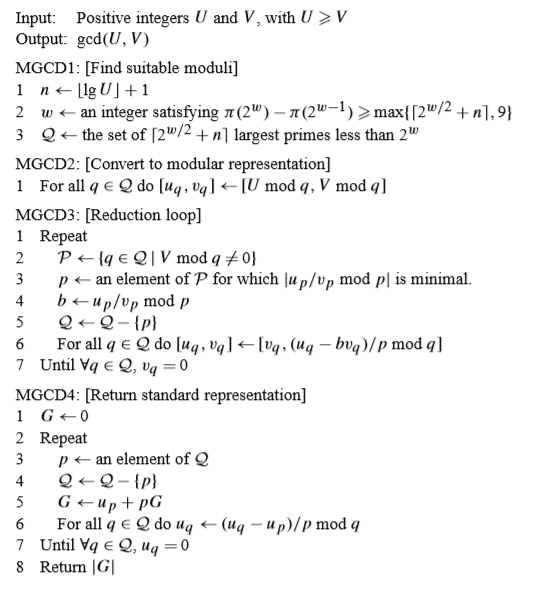
\includegraphics[scale=0.6]{texfiles/integer_mod.PNG}
 \label{fig:ModularAlgorithm}
\end{figure}

The modular algorithm as described by Weber et al.\ is shown in Figure~\ref{fig:ModularAlgorithm}. The algorithm is split into four parts. First, a set of suitable primes $\mathcal{P}$ is selected. Second, the input integers $a$ and $b$ are converted to corresponding modular representations $u_p$ and $v_p$ ($p \in \mathcal{P}$). The third step is the reduction loop. The reduction step is repeated until all $v_p$ are zero. Finally, the result in $u_p$ is transformed back to the standard representation.

The algorithm indicates potential for parallel execution. In particular, the computations of the remainders denoted as \textquote{For all $q \in \mathcal{Q}$ do \dots} in the algorithm can be executed in parallel, making the costly computation of many remainders less time consuming.

\subsection{Implementation}

Both algorithms have been implemented in SageMath as a Jupyter Notebook. The implementations are purely sequential and no efforts have been made in order to utilize the benefit of potential parallel execution so far.

The implementations have been tested thoroughly for various inputs. It was observed that the implementation of the presented modular algorithm did not always yield the correct results. Since we could not find support for the correctness of the backconversion to the standard representation in the proposed algorithm (MGCD4 in Figure~\ref{fig:ModularAlgorithm}), we implemented our own algorithm for the backconversion based on the Chinese remainder algorithm. With this adaption, all our tests passed.

Further, performance tests have been executed in order to demonstrate the better complexity behavior of the modular method. For this purpose, the execution times of both implementations for identical inputs have been measured using Python's timeit function.

\section{Modular GCD of polynomials}\label{Modular GCD of polynomials}

In this section the theory and the algorithm for modular GCD computations for polynomials with one or more variables is described. For this purpose, we employ the algorithm from the book by Franz Winkler~\cite{winkler1996}.

\subsection{Introduction}

Calculating the GCD of polynomials using Euclid's algorithm can lead to large growing coefficients. In order to mitigate this issue, one approach is to make the polynomial monic after each reduction. However, this requires extra integer GCD computations in order to reduce the fractions to the lowest terms. Consequently, the modular GCD algorithm is the method of choice when calculating the GCD of polynomials \cite{modernComputerAlgebra}.

Any modular implementation needs a bound which defines the number of moduli that needs to be taken. 
Depending on the size of the coefficients of the GCD of two polynomials, we need to set a bound which should be derived from the bounds of the coefficients of the input. The coefficient can actually be larger than the coefficients of the input. The GCD of two polynomials $a$ and $b$ needs to be able to divide the leading coefficients $a_m$ and $b_n$ and the degree of the GCD of $a$ and $b$ can not be higher than the minimum degree of $a$ and $b$. 

The bound of the coefficients of the GCD of the two input polynomials \mbox{$a(x) = \sum_{i=0}^m a_i \, x^i$} and \mbox{$b(x) = \sum_{i=0}^n b_i \, x^i$} over $\mathbb{Z}$ ($a_m \neq 0 \neq b_n$ ) is described in absolute value by~\cite{winkler1996}:

\begin{align}
2^{\text{min}(m,n)} \cdot \text{gcd}(a_m, b_n) \cdot \text{min}\left(\frac{1}{|a_m|} \cdot \sqrt{\sum_{i=0}^m a_i^2}, \frac{1}{|b_n|} \cdot \sqrt{\sum_{i=0}^n b_i^2}\right).
\end{align}The bound of the degree of the input polynomials over $F[x]$ can also be used and can be quite sufficient \cite{modernComputerAlgebra}:

\begin{align}
\text{deg}_x \text{gcd}(a, b) \leq \text{min}(\text{deg}_x(a), \text{deg}_x(b).
\end{align}For multivariate polynomials, the bound depending on the degree of the input polynomials can be used~\cite{winkler1996}:

\begin{align}
M = 1 + \text{min}(\text{deg}_x(a), \text{deg}_x(b)).
\end{align}

\subsection{Univariate polynomials}

First, we need to select a set of primes $\mathcal{P}$ which do not divide the leading coefficients of the polynomials $a$ and $b$. Then we need to compute the GCD of $a$ and $b$ modulo every $p$. The GCD of $a$ and $b$ modulo $p$ will have the following properties:

\begin{enumerate}
    \item $\text{deg}(\text{gcd}(a_{p}, b_{p})) \geq \text{ deg}(\text{gcd}(a, b))$
    \item If the resultant of $a / \text{ gcd}(a, b)$ and $b / \text{ gcd}(a, b)$ modulo $p$ is not 0, then $\text{gcd}(a_p, b_p) \equiv \text{ gcd}(a, b) \text{ mod } p$
\end{enumerate}To compute the GCD of two polynomials $a$ and $b$, you need to first compute the Landau-Mignotte bound $M$, then select a prime $p \geq 2 \, M$ which should not divide the leading coefficients of $a$ and $b$. The next step would be to calculate the $\text{gcd}_p$ of $a$ and $b$ modulo $p$. Then you should center the coefficients of the $\text{gcd}_p$ around 0, which will result in values between $-p/2$ and $p/2$, then transform the GCD back to the standard representation and check if it divides $a$ and $b$. If it does, then we have found the GCD. If not, we have chosen an unlucky prime and we need to select another prime and try again. Fortunately, there are only finitely many unlucky primes, so this algorithm will terminate, but it could happen, that $p$ may be very big and the computation may be costly. The algorithm is summarized in Figure~\ref{fig:GCDUni}.

\begin{figure}
\caption{Modular GCD Algorithm for univariate polynomials~\cite{winkler1996}.}
\centering
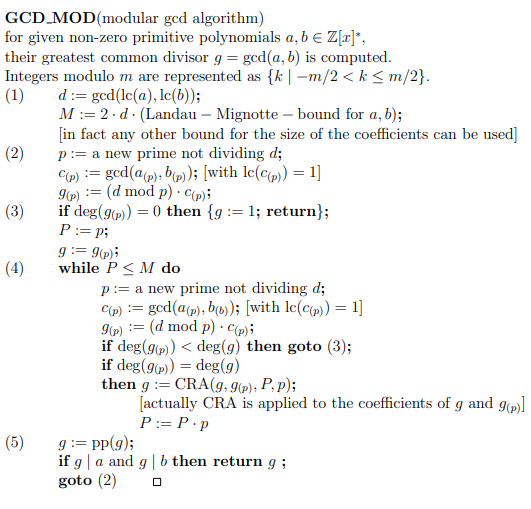
\includegraphics[scale=0.6]{texfiles/polynomial.PNG}
 \label{fig:GCDUni}
\end{figure}

\subsection{Multivariate polynomials}

The polynomials will be described by the form $\mathbb{Z}[x_1 , ... , x_{n-1}][x_n]$, where $x_n$ is the main variable and $\mathbb{Z}[x_1, ..., x_{n-1}]$ are the coefficients. The GCD algorithm for univariate polynomials will be expanded, so that the GCD can be computed for multivariate polynomials. The picked prime will be an irreducible polynomials $p(x)$ in $\mathbb{Z}[x_1, ..., x_{n-1}]$. In fact, this polynomial $p(x)$ will be in the form \mbox{$p(x) = x_{n-1} - r$} with \mbox{$r \in \mathbb{Z}$}. So this will lead to a simple evaluation at $r$ for the reduction modulo $p(x)$. This leads us to the algorithm provided in Figure~\ref{fig:GCDMulti}.

\begin{figure}
\caption{Modular GCD Algorithm for multivariate polynomials~\cite{winkler1996}.}
\centering
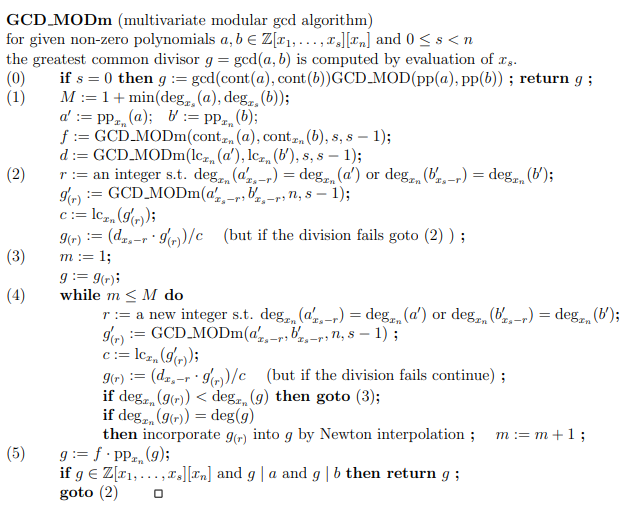
\includegraphics[scale=0.6]{texfiles/multivariate.PNG}
 \label{fig:GCDMulti}
\end{figure}

\section{Results and discussion}\label{results}

In this article, we have demonstrated how the integer GCD can be computed using the modular method. Further, we have discussed the specific benefits and challenges for the modular algorithm.

\begin{table}
    \centering
    \begin{tabular}{rSS}
    \multicolumn{1}{c}{problem size} & \multicolumn{1}{c}{basic algorithm [s]} & \multicolumn{1}{c}{modular algorithm [s]} \\ \hline
         10 & 0.00924 & 0.0244 \\
         20 & 0.0512 & 0.0997 \\
         30 & 0.119 & 0.168 \\
         40 & 0.223 & 0.338 \\
         50 & 0.392 & 0.545 \\
         60 & 0.630 & 0.808 \\
         70 & 0.970 & 1.14 \\
         80 & 1.37 & 1.53 \\
         90 & 1.89 & 1.98 \\
        100 & 2.46 & 2.57 \\
        110 & 3.19 & 3.13 \\
        120 & 3.99 & 3.84 \\
    \end{tabular}
    \caption{Execution times of the basic and the modular integer GCD algorithms for different problem sizes}
    \label{tab:int_results}
\end{table}

In particular, the modular algorithm comes with additional computational overhead, but has a better complexity behavior. This is also confirmed by our performance tests. Table~\ref{tab:int_results} lists the results for the execution times of the basic and the modular integer GCD algorithms for different problem sizes. Apparently, the basic algorithm is significantly faster for small problems. However, going to larger problems, the execution times of the basic algorithm increases dramatically, but not as much for the modular algorithm. From a certain problem size, the modular algorithm outperforms the basic algorithm.

Importantly, these measurements were done without taking advantage of potential parallelization. By utilizing parallel execution, the advantage of the modular algorithm can become even higher.

Furthermore, we have tested the modular approach on univariate and multivariate polynomials. We have demonstrated that the modular method is very useful for implementing a GCD algorithm for polynomials.